%%
%% This is file `sample-manuscript.tex',
%% generated with the docstrip utility.
%%
%% The original source files were:
%%
%% samples.dtx  (with options: `manuscript')
%% 
%% IMPORTANT NOTICE:
%% 
%% For the copyright see the source file.
%% 
%% Any modified versions of this file must be renamed
%% with new filenames distinct from sample-manuscript.tex.
%% 
%% For distribution of the original source see the terms
%% for copying and modification in the file samples.dtx.
%% 
%% This generated file may be distributed as long as the
%% original source files, as listed above, are part of the
%% same distribution. (The sources need not necessarily be
%% in the same archive or directory.)
%%
%% The first command in your LaTeX source must be the \documentclass command.
\documentclass[manuscript,screen, nonacm=true]{acmart}
\usepackage{tikz}
\usepackage{cleveref}
\usepackage{hyperref}
\usepackage{amsmath}
\usepackage{graphicx}
\usepackage{algorithm}
\usepackage[noend]{algpseudocode}

\renewcommand\footnoterule{\kern-3pt \hrule width \textwidth \kern 2.6pt}

%%
%% \BibTeX command to typeset BibTeX logo in the docs
\AtBeginDocument{%
  \providecommand\BibTeX{{%
    \normalfont B\kern-0.5em{\scshape i\kern-0.25em b}\kern-0.8em\TeX}}}

%% Rights management information.  This information is sent to you
%% when you complete the rights form.  These commands have SAMPLE
%% values in them; it is your responsibility as an author to replace
%% the commands and values with those provided to you when you
%% complete the rights form.
\setcopyright{acmcopyright}
\copyrightyear{2018}
\acmYear{2018}
\acmDOI{10.1145/1122445.1122456}

\makeatletter
\let\@authorsaddresses\@empty
\makeatother

\newcommand{\floor}[1]{\left\lfloor #1 \right\rfloor}
\newcommand{\ceil}[1]{\left\lceil #1 \right\rceil}

%%
%% Submission ID.
%% Use this when submitting an article to a sponsored event. You'll
%% receive a unique submission ID from the organizers
%% of the event, and this ID should be used as the parameter to this command.
%%\acmSubmissionID{123-A56-BU3}

%%
%% The majority of ACM publications use numbered citations and
%% references.  The command \citestyle{authoryear} switches to the
%% "author year" style.
%%
%% If you are preparing content for an event
%% sponsored by ACM SIGGRAPH, you must use the "author year" style of
%% citations and references.
%% Uncommenting
%% the next command will enable that style.
%%\citestyle{acmauthoryear}

%%
%% end of the preamble, start of the body of the document source.
\begin{document}

%%
%% The "title" command has an optional parameter,
%% allowing the author to define a "short title" to be used in page headers.
\title{Parallel Smith-Waterman with OpenMP}

%%
%% The "author" command and its associated commands are used to define
%% the authors and their affiliations.
%% Of note is the shared affiliation of the first two authors, and the
%% "authornote" and "authornotemark" commands
%% used to denote shared contribution to the research.
\author{Isitha Subasinghe}
\affiliation{%
  \institution{University of Melbourne}
  \city{Melbourne}
  \state{Victoria}
  \country{Australia}
}
\email{isubasinghe@student.unimelb.edu.au}


%%
%% By default, the full list of authors will be used in the page
%% headers. Often, this list is too long, and will overlap
%% other information printed in the page headers. This command allows
%% the author to define a more concise list
%% of authors' names for this purpose.
\renewcommand{\shortauthors}{}

%%
%% The abstract is a short summary of the work to be presented in the
%% article.
\begin{abstract}
  Sequence alignment is the process of comparing and detecting similarities in biological sequences such as 
  RNA and DNA. The idiomatic algorithm presented for this problem is inherently sequential. This report explores how the problem may be parallelised using the "wavefront" technique along with OpenMP \footnote{See \url{https://www.openmp.org}} . The algorithm implemented using OpenMP was able to offer a speedup of 13 over the sequential algorithm, interestingly, the effeciency of adding more cores to the problem was shown to decrease exponentially. 
\end{abstract}

%%
%% The code below is generated by the tool at http://dl.acm.org/ccs.cfm.
%% Please copy and paste the code instead of the example below.
%%
\begin{CCSXML}
	<ccs2012>
	<concept>
	<concept_id>10010147.10010169.10010170</concept_id>
	<concept_desc>Computing methodologies~Parallel algorithms</concept_desc>
	<concept_significance>500</concept_significance>
	</concept>
	</ccs2012>
\end{CCSXML}

\ccsdesc[500]{Computing methodologies~Parallel algorithms}


%%
%% This command processes the author and affiliation and title
%% information and builds the first part of the formatted document.
\maketitle

\section{Background}
The Smith-Waterman \cite{smith1981identification} algorithm introduced about 40 years ago, is the only known algorithm that is able to find the optimal local alignment of sequences, however, it is also one of the slowest algorithms for sequence alignment. With the exponential growth of biological databases, far outpacing microprocessor improvements, the use of parallelism to speed up the Smith-Waterman algorithm is of importance to bioinformatics. The algorithm itself is not trivially parallelisable, however, recognising the dependencies for the values in the dynamic programming matrix helps in observing that the algorithm is still however, parallelisable. The dependencies of the values in the dynamic programming matrix are shown in \cref{fig:smiwatdeps}.
\begin{figure}[!h]
\centering
    \begin{tikzpicture}[scale=1]
    \clip (-0.3,-1.3) rectangle (8.3,4.3);
%   \foreach \x in {0,...,8} {
%       \foreach \y [evaluate=\y as \z using int(4-\y)] in {0,...,4} {
%           \pgfmathtruncatemacro{\myresult}{\x<\z ? 1 : 0}
%           \ifnum\myresult=0%
%           \node at (\x cm,\y cm) (g-\x-\y) {$a_{\x,\z}$};\fi
%       }
%   }
    \foreach \x in {0,...,8} {
      \foreach \y [evaluate=\y as \z using int(4-\y)] in {0,...,4} {
        \node at (\x cm,\y cm) (g-\x-\y) {$d_{\x,\z}$};
      }
    }
    % vertical dependency
    \foreach \x in {1,...,8} {
      \foreach \y in {0,...,3} {
        \draw[<-] (g-\x-\y) -- +(0,20pt);
      }
    }
    % horizontal
    \foreach \x in {0,...,7} {
      \foreach \y in {0,...,3} {
        \draw[->] (g-\x-\y) -- +(20pt,0);
      }
    }
    % diagonal
    \foreach \x in {1,...,8} {
      \foreach \y in {0,...,3} {
        \draw[<-] (\x-.3,\y+.3) -- (\x - .6, \y+.6);
      }
    }
    \end{tikzpicture}
\caption{Dependencies for values in Smith-Waterman matrix}
\label{fig:smiwatdeps}
\end{figure}

\section{Related Work}
Searching of DNA and RNA sequences is a fundamental task in bioinformatics and as mentioned previously Smith-Waterman offers optimal local alignment. However, as a result of optimal local alignment being computationally expensive, the most common solutions do not aim to provide this, instead they use heuristics to reduce the computational cost, examples of such tools are FASTA \cite{pearson1988improved} and BLAST \cite{altschul1997gapped}.

Early work in parallelising Smith-Waterman was based upon diagonal parallelisation, this was initially done through SIMD instructions.SIMD implementations have proven to be popular as a result of their common availability in x86 systems and have demonstrated significant speedups in several published literature \cite{rognes2000six, zhao2013ssw}.  

With the rapid accessibility of GPUs over the years following the early work on SIMD parallelism, CUDA compatible GPUs were found to be effective as hardware accelerators for the local optimal alignment problem. The CUDA implementation shown in \cite{manavski2008cuda} was demonstrated to be 2 to 30 times faster than other implementations on commodity hardware at the time. 

Field Programmable Gate Arrays are integrated circuits that can be programmed through the user, using some hardware description language such as VHDL or Verilog. These implementations are naturally faster than their counterparts in higher level languages as the circuit itself is programmed for the specific problem, however, they are difficult to program and debug. Storaasli \cite{storaasli2007accelerating} claims that their implementation of Smith-Waterman on two Cray XD1 systems was able to obtain a 100x speedup. Interestingly, speedups of 160x have been made through the use of FPGAs as shown in \cite{li2007160}.

\section{Proposed Approach}


\subsection{Sequential Algorithm}
The sequential algorithm used was near identical to the provided program, however certain optimisations were performed to the program, along with bug fixes. The code for this algorithm is shown below:
\begin{algorithm}
\caption{Sequential Smith-Waterman}\label{alg:naive}
\begin{algorithmic}[1]
\Procedure{SeqSmithWaterman}{}
\State $\text{m,n} \gets \text{dimensions of }\textit{matrix}$
\State $pgap \gets \textit{gap penalty}$
\State $pxy \gets \textit{mismatch penalty}$
\State $\text{dp[m][n]} \gets \text{newMatrix(m+1,n+1)}$
\State $\text{x} \gets \textit{sequence x}$
\State $\text{y} \gets \textit{sequence y}$
\For{$\text{i} \gets [0 \ldots m] $}
    \State $\text{dp[i][0]} \gets \text{i} * \text{pgap}$
\EndFor
\For{$\text{i} \gets [0 \ldots n] $}
    \State $\text{dp[0][i]} \gets \text{i} * \text{pgap}$
\EndFor
\For{$\text{i} \gets [1 \ldots m]$}
    \For{$\text{j} \gets [1 \ldots n]$}
    	\If{$\text{x[i-1]} = \text{y[j-1]}$}
    		\State $\text{dp[i][j]} = \text{dp[i-1][j-1]}$
    	\Else
    		\State $\text{dp[i][j]} = \text{min(dp[j-1][i-1] + pxy, dp[j-1][i] + pgap, dp[j][i-1] + pgap)}$
    	\EndIf
    \EndFor
\EndFor
\textbf{return } \text{traceback(dp)}
\EndProcedure
\end{algorithmic}
\end{algorithm}

\subsection{Parallel Algorithm}
The psuedocode for the parallel algorithm is defined as follows:


\begin{algorithm}
\caption{Parallel Smith-Waterman}\label{alg:parsmith}
\begin{algorithmic}[1]
\Procedure{ParSmithWaterman}{}
\State $\text{m,n} \gets \text{dimensions of }\textit{matrix}$
\State $pgap \gets \textit{gap penalty}$
\State $pxy \gets \textit{mismatch penalty}$
\State $\delta_i \gets \textit{tile width}$
\State $\delta_j \gets \textit{tile height}$
\State $outer_i \gets 0$
\State $outer_j \gets 0$
\State $diagonals \gets \floor{\frac{m}{\delta_i}} + \floor{\frac{n}{\delta_j}} + \begin{cases} 
      1 & m\%\delta_i + n\%\delta_j > 0 \\
      0 & m\%\delta_i + n\%\delta_j = 0 \\
    \end{cases}$
\State $\text{dp[m][n]} \gets \text{NewMatrix(m+1,n+1)}$
\State $\text{x} \gets \textit{sequence x}$
\State $\text{y} \gets \textit{sequence y}$
\For{$\text{i} \gets [0 \ldots m] \textbf{ parallel} $}
    \State $\text{dp[i][0]} \gets \text{i} * \text{pgap}$
\EndFor
\For{$\text{i} \gets [0 \ldots n] \textbf{ parallel}$}
    \State $\text{dp[0][i]} \gets \text{i} * \text{pgap}$
\EndFor
\For{$\text{i} \gets [0 \ldots diagonals)$}
    \State $diff_i \gets outer_i$
    \State $diff_j \gets n-outer_j-1$
    \State $diag_i \gets 1 + \floor{\frac{diff_i}{\delta_i}}$
    \State $diag_j \gets 1 + \floor{\frac{diff_j}{\delta_j}}$
    \State $length \gets min(diag_i, diag_j)$
    \For{$\text{tile} \gets [0 \ldots length) \textbf{ parallel} $}
        \State $inner_i \gets max(1, outer_i - (tile*\delta_i))$
        \State $inner_j \gets max(1, outer_j + (tile*\delta_j))$
    	\State $imax \gets max(inner_i + \delta_i, width)$
    	\State $jmax \gets max(inner_j + \delta_j, height)$
    	\For{$\text{i} \gets [inner_i \ldots imax]$}
            \For{$\text{j} \gets [inner_j \ldots jmax]$}
        	    \If{$\text{x[i-1]} = \text{y[j-1]}$}
        		    \State $\text{dp[i][j]} = \text{dp[i-1][j-1]}$
        	    \Else
        		    \State $\text{dp[i][j]} = \text{min(dp[j-1][i-1] + pxy, dp[j-1][i] + pgap, dp[j][i-1] + pgap)}$
        	    \EndIf
            \EndFor
        \EndFor
    \EndFor
    \If{$outer_i + \delta_i < m$}
        \State $outer_i \gets outer_i + \delta_i$
    \Else
        \State $outer_j \gets outer_j + \delta_j$
    \EndIf
\EndFor
\textbf{return } \text{traceback(dp)}
\EndProcedure
\end{algorithmic}
\end{algorithm}

\clearpage 

\subsubsection{Restrictions}
There was a restriction in the implementation of our algorithm, namely the amount of memory available proved constraining in exploiting further opportunities for parrallelism. Computing the sequence alignment among all $\frac{k(k-1)}{2}$ pairs is ``embarrassingly parallel'', however, this leads to far greater memory consumption and therefore wasn't a valid optimisation given our memory restrictions. 

\subsubsection{NUMA awareness}
NUMA (non-uniform memory access) becomes an area of concern when considering programs that use multiple cores. 
More accurately, when multi-core programs require access to the same memory locations as each other and this sharing is performed over an interconnect. 
The policy used to help reduce the cost of NUMA in the Parallel implementation is called ``First Touch''.
``First Touch'' ensures that the NUMA node to initialise some memory location, will have that page allocated on a memory device physically closer to the NUMA node.\\
The steps for memory allocation can be given as follows:
\begin{itemize}
	\item dynamic memory allocation call (malloc/new)
	\item initial write attempt of dynamically allocated memory
	\item page fault triggered when write is attempted
	\item physical allocation of memory performed and mapped via MMU
\end{itemize}
The parallel implementation exploits this property on moderns operating systems to help reduce the cost of non-uniform memory access. This is performed by initialising the
matrix used for Smith-Waterman through multiple threads, ensuring that each NUMA node has a slice of the memory and thus a lower number of memory transfers are done over the interconnect, this is shown in \cref{alg:parnewmatrix}. 

While this is helpful for distributing the pages among the NUMA nodes, it comes at an additional processing cost. With the GNU 11.1.0 compiler toolchain, we are able to make use of the OpenMP allocator to do this distribution of pages, additionally some further optimisations maybe performed to increase performance, such as removing thread safety from the allocator and ensuring that the allocated memory is aligned, aligning memory is useful when using SIMD as load operations are much faster. 


\subsubsection{Optimum tile size}
The tile size presents a significant influence on the speedup of our algorithm, along with the scheduling algorithm used. The intuition regarding the dimensions of the tile size maybe to minimise it as much as possible, however, this is not always the optimial strategy. Likewise, it may seem that static scheduling maybe the most sensible given that each core would perform relatively the same amount of work, however, this is also untrue. A deeper discussion regarding the scheduling of wavefront parallelism on shared memory multiprocessors is provided in \cite{manjikian1996scheduling}. In our implementation, the tile size was determined by dividing the dimensions by a fixed number and the scheduling was performed dynamically, these details were determined through experimentation. 

\subsubsection{Cache optimisations}
Memory latencies play a significant role in the performance of programs, ensuring false sharing is minimal and maintaining locality of reference are important objectives for any high performance application. The processing of tiles in the wavefront processing of the matrix, helps obtain the previously mentioned objectives as shown by \cite{manjikian1996scheduling}. This is as a result of the layout of memory used in the matrix itself, the entire matrix is allocated as a single contiguous slice of memory. Consider the parallel traversal of the yellow diagonals below in \cref{fig:diag}. An isolated view of the potential cache lines for each core is also visible in \cref{fig:cachelines}, observe how given sufficient width of the matrix, false sharing is extremely unlikely. Additionally, note how the tiles are traversed horizontally and then vertically, this maintains locality of reference as the rows are contiguous in memory which is crucial to high performant code. 

\begin{figure}[h]
    \centering
    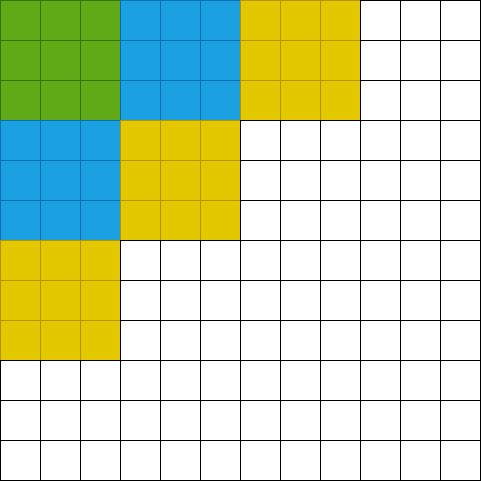
\includegraphics[scale=0.25]{diag}
    \caption{Parallel processing of diagonals}
    \label{fig:diag}
\end{figure}
\begin{figure}[h]
    \centering
    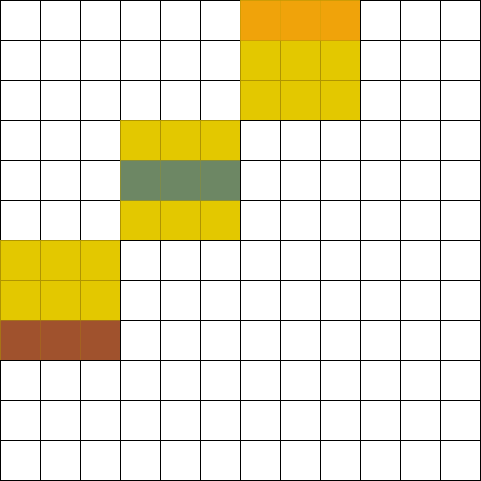
\includegraphics[scale=0.25]{cachelines}
    \caption{Potential cache lines}
    \label{fig:cachelines}
\end{figure}

\subsubsection{Compiler optimisations}
Compiler optimisations were heavily used to further increase the performance of the algorithm and frequent profiling of the program was done via the linux utility ``perf`` \footnote{See \url{https://perf.wiki.kernel.org/index.php/Main_Page}}. It is important to note that using ``std::string'' had a significant impact on performance when dynamically linked to our program, this is as a result of symbol lookup performed in a tight loop when traversing the dynamic programming matrix. The remedy was to statically link the C++ standard library, which lead to a significant increase in performance, almost exactly the same performance characteristics as using a simple character array for holding the sequences. Additional optimisation recommendations from \cite{fog2020optimizing} were evaluated and used where appropriate. A critical optimisation used was the ``-march=native'' flag passed onto the GNU compiler, this flag targets the exact architecture that we are compiling the program for, this results in further architecture level optimisations being possible such as usage of AVX-512 \footnote{See \url{https://www.intel.com.au/content/www/au/en/architecture-and-technology/avx-512-overview.html}}.

\section{Experiments}

\subsection{Experiment Environment}
Two experimentation environments were used throughout the development process. The development environment was used as a quick way to test and filter out
ideas that weren't viable, while valid ideas were tested on the Spartan High Performance Computing cloud \cite{lafayette2017hpc}. 
\subsubsection{Development Environment}
\begin{itemize}
    \item CPU - AMD Ryzen™ 7 3700X @ 3.6-4.4GHz
    \item Memory - 32GB
    \item Compiler - GNU 11.1.0
\end{itemize}

\subsubsection{Spartan Environment}
\begin{itemize}
    \item CPU - Intel(R) Xeon(R) Gold 6154 CPU @ 3.00-3.7GHz
    \item Memory - 32GB 
    \item Compiler - GNU 10.3.0
\end{itemize}




\subsection{Results}
The results after running our parallel algorithm on the ``mseq-big13-example'' data provided are shown in \cref{fig:results} and presented in below in \cref{table:results}. 
\begin{figure}[!ht]
    \centering
    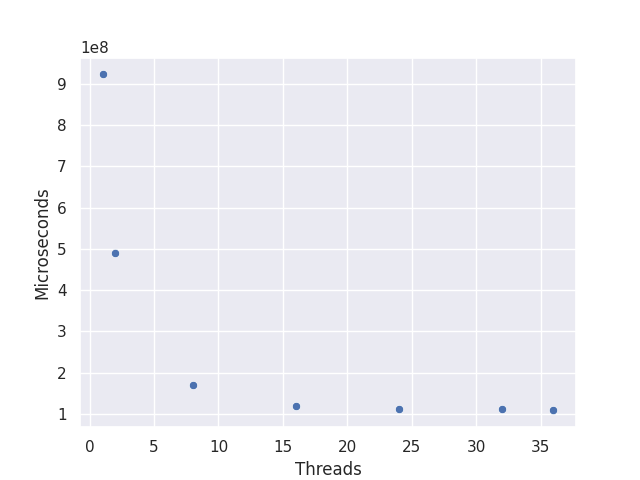
\includegraphics[scale=0.6]{res}
    \caption{Results observed}
    \label{fig:results}
\end{figure}
% y = [923129129, 491227097, 169576852, 119517599, 112753964, 111237046, 108483498]

\begin{table}[!h]
    \begin{tabular}{||c|c||}
        \hline
        Core(s) & Walltime(microseconds) \\ \hline
        1       & 923129129 $\mu s$ \\ 
        \hline
        2       & 491227097 $\mu s$ \\
        \hline
        8       & 169576852 $\mu s$ \\
        \hline
        16      & 119517599 $\mu s$ \\
        \hline
        24      & 112753964 $\mu s$ \\
        \hline
        32      & 111237046 $\mu s$ \\
        \hline
        36      & 108483498 $\mu s$ \\
        \hline
    \end{tabular}
    \label{table:results}
    \caption{Walltime per number of cores}
\end{table}


\subsection{Determining Efficiency}
The efficiency( $\eta(n)$ ) of our algorithm can be determined by the following formula: 
\begin{equation}
    \eta(n) = \frac{\text{Speedup(n)}}{\text{p(n)}}
    \label{eq:efficiency}
\end{equation}
The efficiency for the results shown in \cref{table:results} have been calculated using \cref{eq:efficiency} and displayed in \cref{table:efficiency}. 

\begin{table}[!h]
    \begin{tabular}{||c|c||}
        \hline
        Core(s) & Efficiency \\ \hline
        1       & 1.572  \\ 
        \hline
        2       & 1.478 \\
        \hline
        8       & 1.070 \\
        \hline
        16      & 0.759 \\
        \hline
        24      & 0.537 \\
        \hline
        32      & 0.408 \\
        \hline
        36      & 0.372 \\
        \hline
    \end{tabular}
    \label{table:efficiency}
\end{table}



\subsection{Exploring implications of tile size}

\begin{table}[!h]
    \begin{tabular}{||c|c|c||}
        \hline
        Core(s) & Tile Size & Walltime(microseconds) \\ \hline
        8       &  $(\frac{m}{8} + 1, \frac{n}{8}+1)$  & 379606318 $\mu s$ \\ 
        \hline
        16       &  $(\frac{m}{16}+1, \frac{n}{16}+1)$  & 382288384 $\mu s$ \\
        \hline
        24       &  $(\frac{m}{24}+1, \frac{n}{24}+1)$  & 388430562 $\mu s$ \\
        \hline
        32     &  $(\frac{m}{32}+1, \frac{n}{32}+1)$ & 385640454 $\mu s$ \\
        \hline
        36      & $(\frac{m}{36}+1, \frac{n}{36}+1)$ & 381233563 $\mu s$ \\
        \hline
    \end{tabular}
    \label{table:tileresults}
    \caption{Walltime per number of cores and tile size}
\end{table}

\subsection{Discussion}
\textbf{Note: } The sequential implementation was measured to have taken 1451965419 $\mu s$.
\vspace{2mm}
\\
The results were extremely surprising, note that the single core parallel algorithm is far more performant than the sequential algorithm. While this was unexpected, this is likely due to the substantial amount of micro optimisations and time spent on the implementation of the parallel algorithm itself rather than the complexity properties of the parallel algorithm itself. 
\vspace{2mm}
\\
The choice of cores to test were not random, they were also made with the intention of determining the effectiveness of our NUMA mitigation strategy mentioned previously. The processor used consisted of 18 cores, this fact ensures that when the core count requested is above 18, we are guaranteed to encounter at least two NUMA nodes. Note that, in practice, this number was in fact much higher at 3-5 NUMA nodes per experiment. The results in \cref{table:results} show that our NUMA mitigation strategy was effective, although NUMA certainly would have contributed in adding latencies to our calculations as our core count went up, the increase in parallelism was able to counteract this. The decrease in efficiency as core count increased,  demonstrated in \cref{table:efficiency} is likely a function of NUMA costs and the limit on the parallelisability of the problem itself. 
\\
\\
As stated previously, the tile size has a significant impact on the parallelisability of the problem. As shown in \cref{table:tileresults}, choosing a bad tile size may mean the parallelisability of the problem is artificially limited. The results in \cref{table:results}, \cref{fig:results} and \cref{table:efficiency} are a result of dynamically choosing the tile size based on the dimensions of the matrix. To be exact, the dimensions of the matrix were divided by 13, determining this number was through experimentation on the development environment. 

\section{Further Work}
\subsection{Generation of tiles}
The parallel algorithm implemented does not make full use of the available computing power. When tiles are iterated over, they must wait until all the tiles in the same diagonal have completed their work. This is an unnecessary restriction, as it results in a large amount of time spent on the barrier.
Further work could explore how to reduce the level of granularity in our dependencies, new tiles could simply be generated after a single tiles work unit has completed. A simple algorithm would be to start processing tile $(i+\delta_i,j)$ and $(i,j+\delta_j)$ when $(i,j)$ has completed its unit of work, this does however introduce the problem of tiles being visited more than once but this could simply be avoided through using a xorfilter to determine if a pair of indices have been visited before.

\subsection{Inter-sequence SIMD parallelism}
We could apply inter-sequence SIMD parallelism into our current thread-parallel implementation to obtain instruction level parallelism. 
While this is plausible, an important consideration that warrants investigation is determining an efficient method to move data from the heap and into the SIMD register, this technique will likely have significant speedups with AVX-512. 

\section{Conclusion}
We have demonstrated how OpenMP may be used to develop a parallel algorithm for optimal local alignment of sequences. The algorithm developed showed effective use of parallelism to achieve a significant speedup of 13 over the sequential algorithm. 

\nocite{lameter2013overview}

\bibliographystyle{ACM-Reference-Format}
\bibliography{sample-base}



\appendix
\section{Appendix}

\begin{algorithm}
	\caption{Parallel Matrix initialisation}\label{alg:parnewmatrix}
	\begin{algorithmic}[3]
		\Procedure{NewMatrix}{}
		\State $\text{m,n} \gets \text{dimensions of }\textit{matrix}$

		\State $\text{dp} \gets \text{malloc(sizeof(int *)*m)}$
		\State $\text{size} \gets \textit{m*n}$
		\State $\text{dp0} \gets \text{malloc(sizeof(int)*size)}$
		
		\For{$\text{i} \gets [0 \ldots \text{size}) \textbf{ parallel} $}
			\State $\text{dp0[0]} \gets 0$
		\EndFor
		\For{$\text{i} \gets [0 \ldots m) \textbf{ parallel} $}
			\State $\text{dp[0]} \gets 0$
		\EndFor
		
		\State $\text{dp[0]} \gets \text{dp0}$
		
		\For{$\text{i} \gets [1 \ldots m) $}
		\State $\text{dp[0]} \gets \text{dp[i-1] + n}$
		\EndFor
		
		\State $\textbf{return } \text{dp}$
		\EndProcedure
	\end{algorithmic}
\end{algorithm}


\end{document}
\endinput
%%
%% End of file `sample-manuscript.tex'.
